\section{Kupplungen}

\subsection{Einscheibenkupplungen}
\begin{vardef}
	\item[$R_\text{a}$] Außenradius der Kupplungsscheibe
	\item[$R_\text{i}$] Innenradius der Kupplungsscheibe
	\item[$S$] Axiale Betriebskraft
	\item[$d_\text{m}$] Mittlerer Durchmesser der Kupplungsscheibe
	\item[$b$] Breite der Kupplungsscheibe
\end{vardef}

\begin{figure}[H]
	\centering
	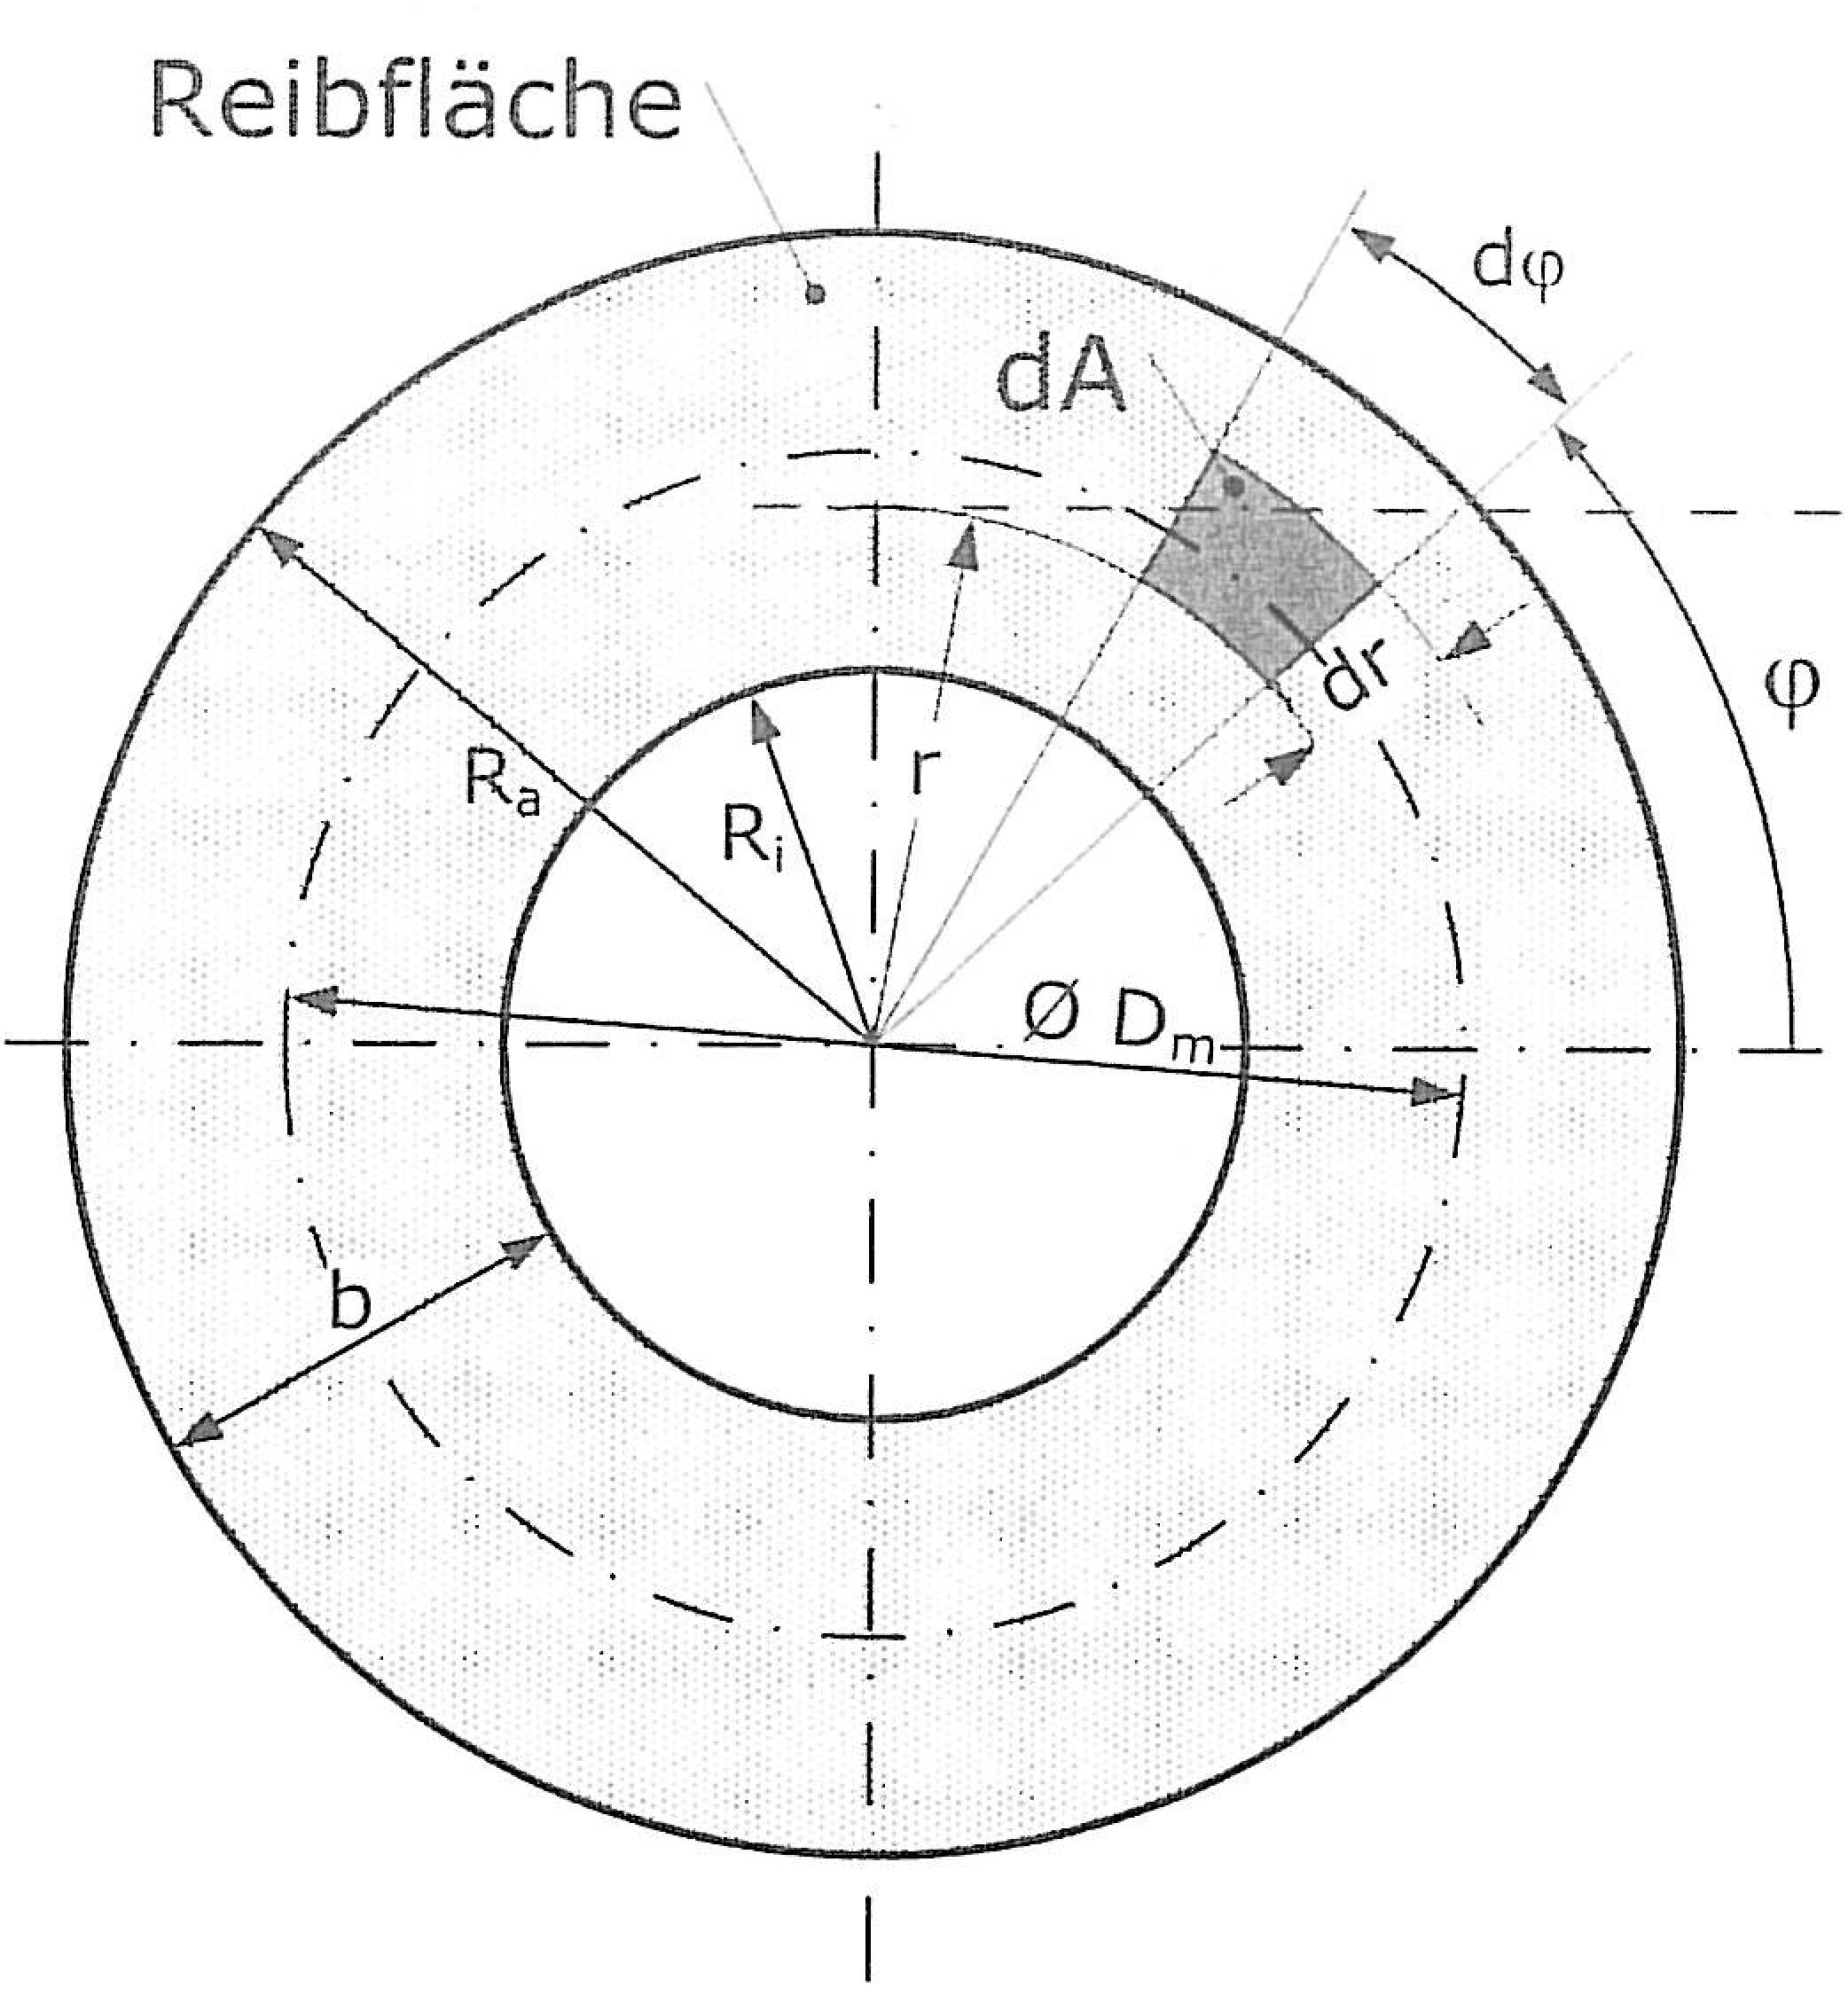
\includegraphics[width=0.35\linewidth]{kupplungen/einscheibenkupplung.jpg}
	\caption*{Geometrie der Kupplung}
\end{figure}

% Hilfsgrößen
\hrule
\begin{eeqn}{Hilfsgrößen}
	\begin{align}
		&b = \frac{D_\text{a}-D_\text{i}}{2} = R_\text{a} - R_\text{i}  \\
		&d_\text{m} = \frac{D_\text{A}+D_\text{i}}{2} =R_\text{a} + R_\text{i}
	\end{align}
\end{eeqn}

% Moment im Neuzustand der Kupplung
\begin{eeqn}{Moment im Neuzustand der Kupplung}
	\begin{align}
		M &= \frac{2\cdot S \cdot \mu}{3 \cdot d_\text{m} \cdot b} \cdot \left( R_\text{a}^3 - R_\text{i}^3\right)
	\end{align}
\end{eeqn}

% Moment im Gebrauchtzustand der Kupplung
\begin{eeqn}{Moment im Gebrauchtzustand der Kupplung}
	\begin{align}
		M &= S \cdot \mu \cdot \frac{d_\text{m}}{2}
	\end{align}
\end{eeqn}

% Auslegung von Kupplungen
\begin{eeqn}{Auslegung von Kupplungen}
	Kupplungen werden immer auf den Gebrauchtzustand ausgelegt, anschließend wird dann das Moment im Neuzustand überprüft. \\
	Wenn bei der Kupplung $N$ Reibflächen entstehen, gilt für das gesamte übertragbare Moment $M_\text{zul}$:
	\begin{align}
		M_\text{ges} = N \cdot M
	\end{align}
\end{eeqn}

\subsection{Kegelpressverbindungen}
\begin{vardef}
	\item[$\beta$] Halber Öffnungswinkel des Kegels
	\item[$D_\text{m}$] Mittlerer Durchmesser des Kegels
	\item[$S_\text{E}$] Anpresskraft des Kegels
	\item[$L$] Länge des Kegels
\end{vardef}

\begin{figure}[H]
	\centering
		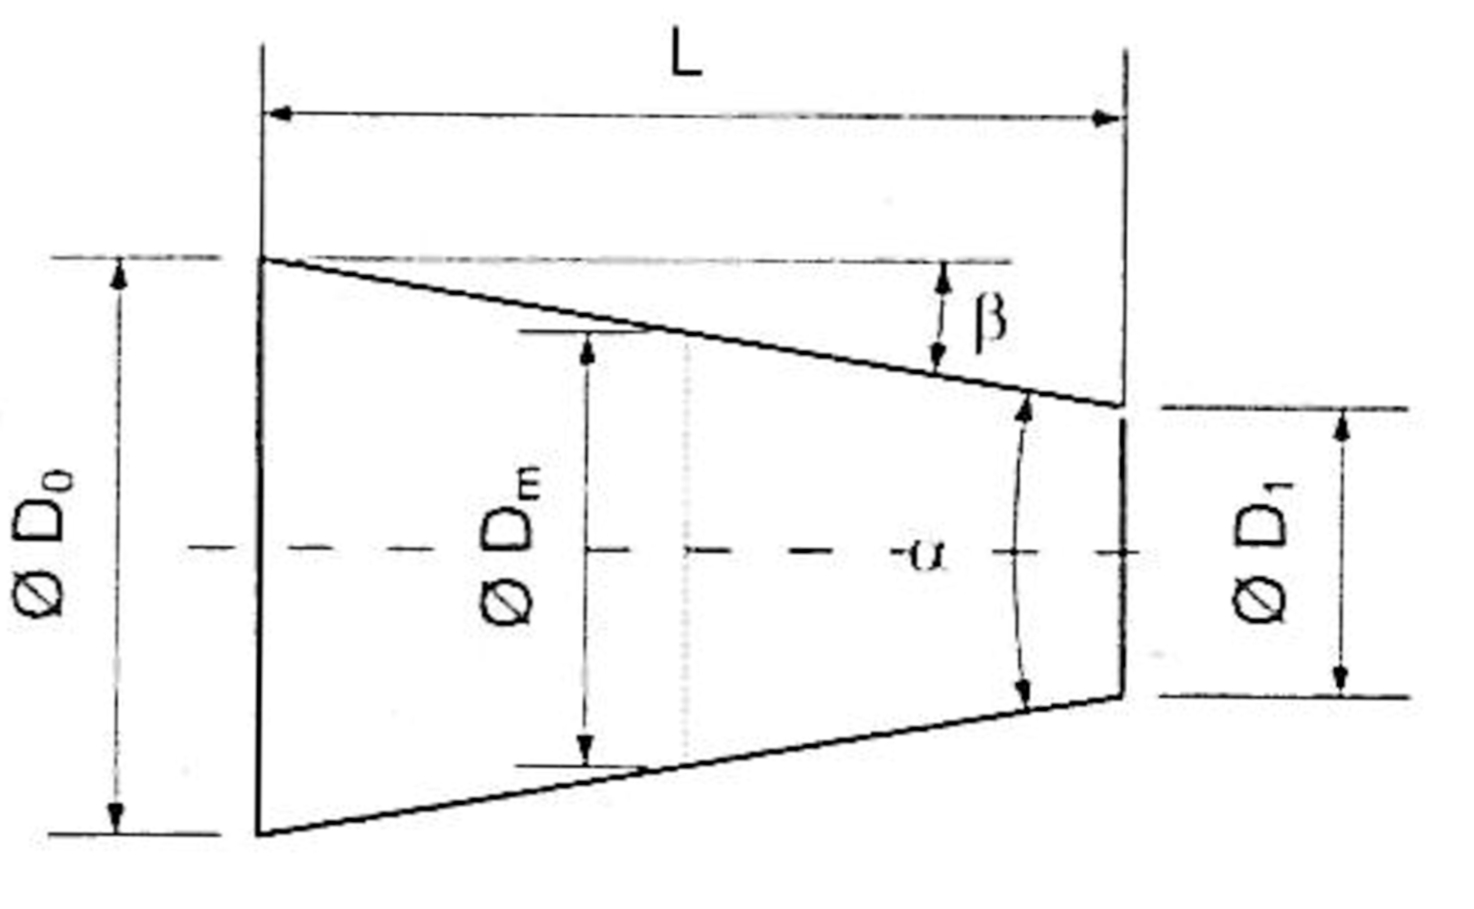
\includegraphics[width=0.6\linewidth]{kupplungen/kegel-welle}
		\caption*{Geometrie des Kegels}
		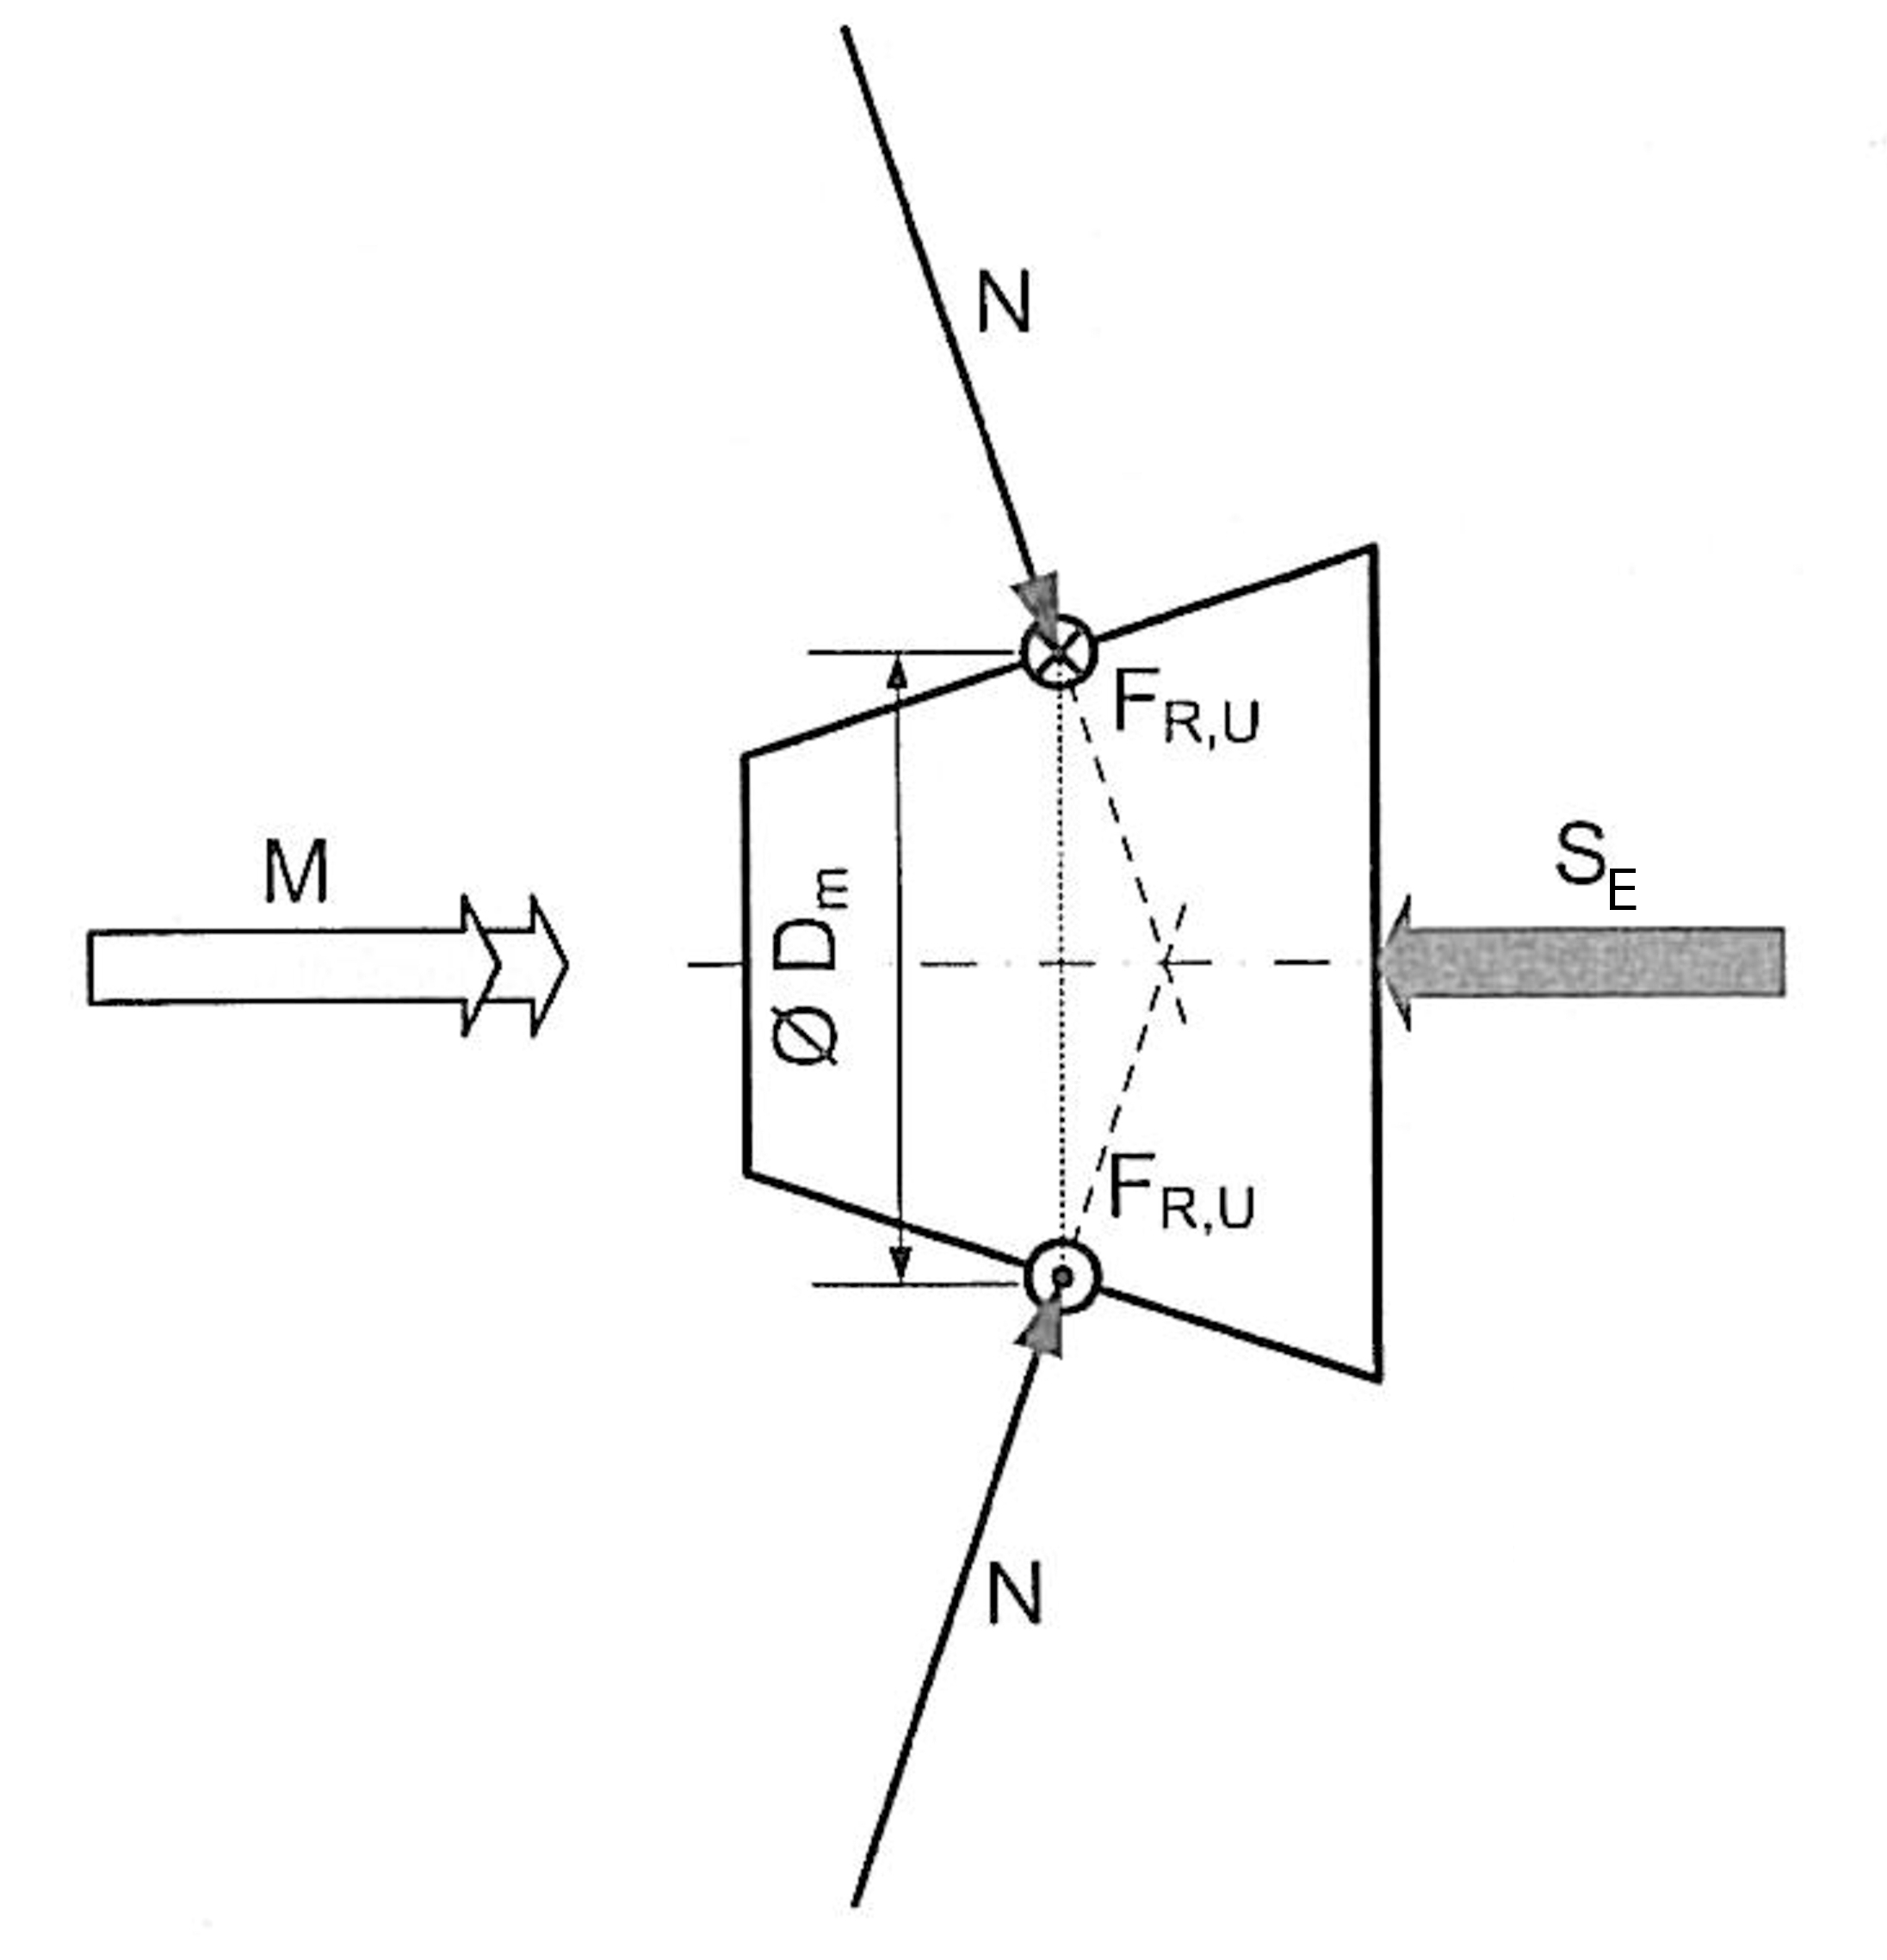
\includegraphics[width=0.6\linewidth]{kupplungen/kegel-welle-frei}
		\caption*{Krafteinwirkung auf den Kegel}
\end{figure}

% Mittlerer Durchmesser
\begin{eeqn}{Mittlerer Durchmesser}
	\begin{align}
		D_\text{m} &= \frac{D_0+D_1}{2}
	\end{align}

\end{eeqn}

% Kegelverhältnis
\begin{eeqn}{Kegelgeometrie}
	Kegelverhältnisse werden als $\rhd\;x:y$ angegeben. Dies entspricht:
	\begin{align}
		C & = \frac{x}{y} = \frac{D_0-D_1}{L}
	\end{align}
	Beispiel: $\rhd\; 1:10 \Rightarrow C=0,1$ \\
	Um den halben Öffnungswinkel $\beta$ zu erhalten nutzt man:
	\begin{align}
		\beta & = \arctan \frac{C}{2}
	\end{align}
\end{eeqn}

% Übertragbares Drehmoment
\begin{eeqn}{Übertragbares Drehmoment}
	\begin{align}
		M &= \frac{S_\text{E} \cdot \mu \cdot D_\text{m}}{2\cdot (\sin \beta + \mu \cdot \cos \beta)}
	\end{align}
	Auslegungsgleichung für Kegel-Welle Verbindungen
\end{eeqn}

% Kegelpressung
\begin{eeqn}{Kegelpressung}
	\begin{align}
		P &= \frac{2\cdot M \cdot \cos \beta}{\mu \cdot \pi \cdot L \cdot D_\text{m}^2}
	\end{align}
	Pressung in der Fuge einer Kegel-Welle Verbindung
\end{eeqn}
\vfill
\pagebreak

\subsection{Klemmverbindungen}
\begin{vardef}
	\item[$D_\text{F}$] Durchmesser der Fuge
	\item[$D_\text{B}$] Bohrungsdurchmesser für die Schraube
	\item[$F_\text{N}$] Gesamte Radiale Spannkraft
	\item[$H$] Höhe der Klemmverbindung
\end{vardef}

% geteilte (biegesteife) Klemmverbindung
\hrule
\begin{eeqn}{geteilte (biegesteife) Klemmverbindung}
	\begin{align}
		M &= \mu \cdot F_\text{N} \cdot D_\text{F}
	\end{align}
	Die Klemmen werden bei diesem Typ auf Spielpassung ausgelegt. Die Krafteinleitung erfolgt über zwei Punkte.
\end{eeqn}

% geteilte (biegeweiche) Klemmverbindung
\begin{eeqn}{geteilte (biegeweiche) Klemmverbindung}
	\begin{align}
		M &= \mu \cdot F_\text{N} \cdot D_\text{F} \cdot \frac{\pi}{2}
	\end{align}
	Die Klemmen werden bei diesem Typ auf Presspassung ausgelegt. Die Krafteinletung erfolgt über die gesamte Mantelfläche der Welle.
\end{eeqn}

\begin{figure}[H]
	\centering
	\begin{minipage}[b]{0.49\linewidth}
		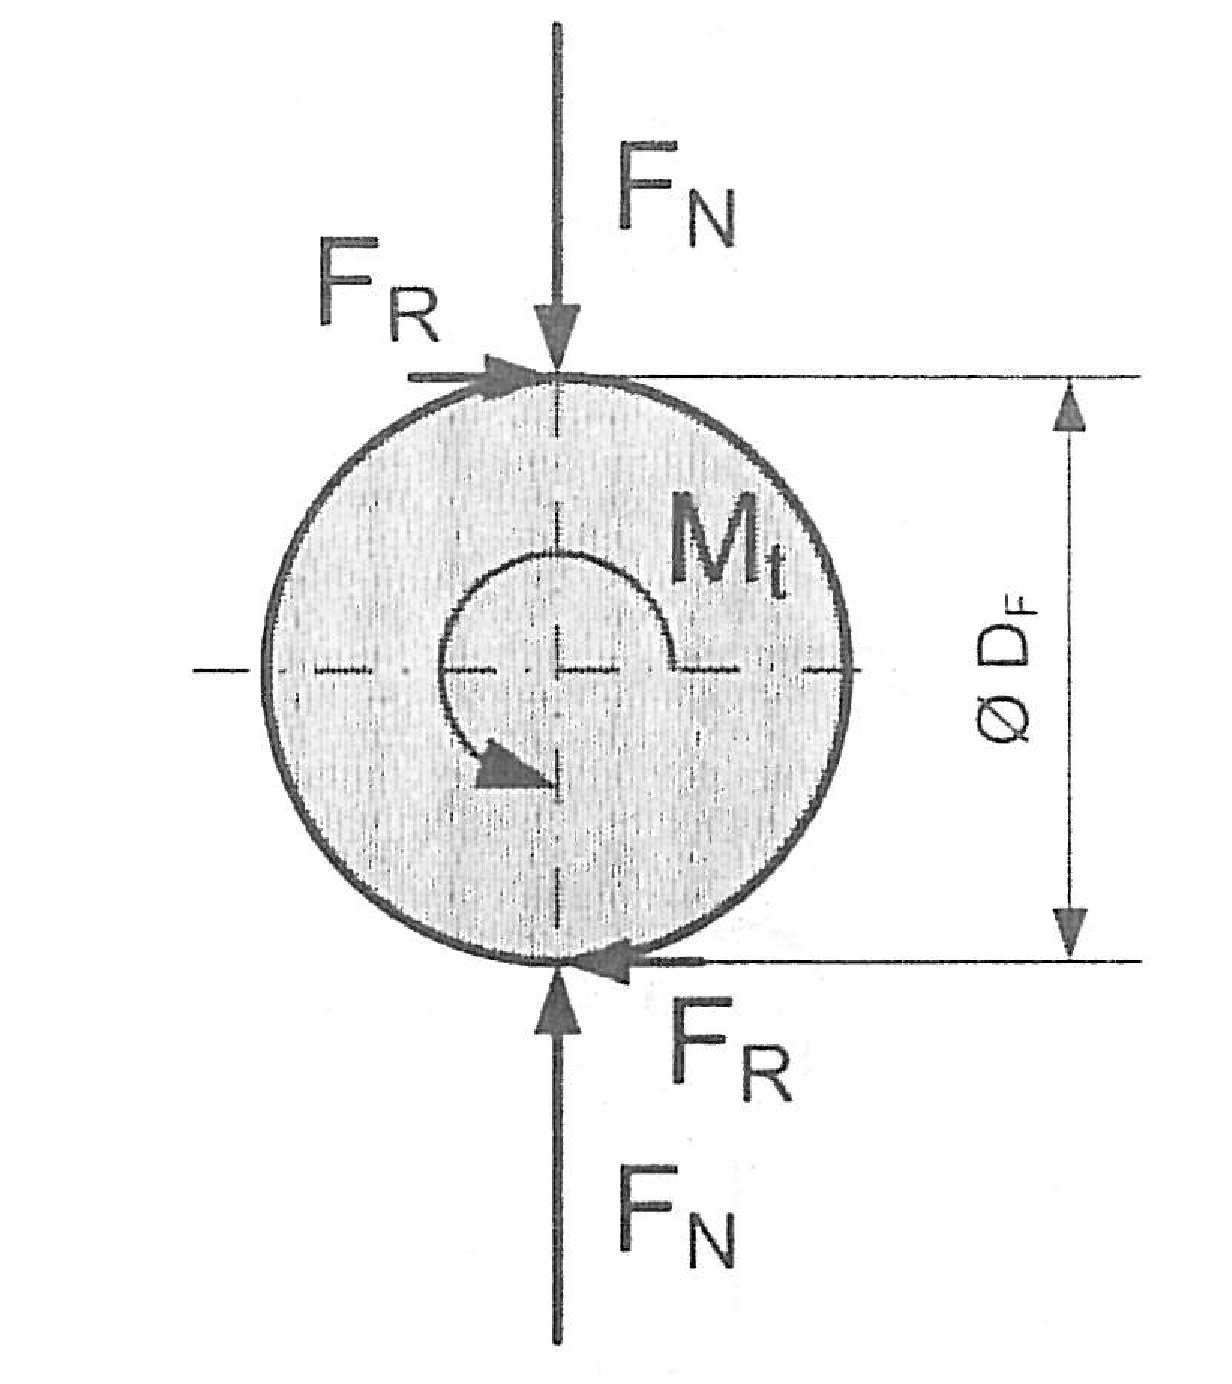
\includegraphics[width=\linewidth]{kupplungen/klemmverbindung-starr}
		\caption*{Biegestarre Klemmverbindung}
	\end{minipage}
		\begin{minipage}[b]{0.49\linewidth}
		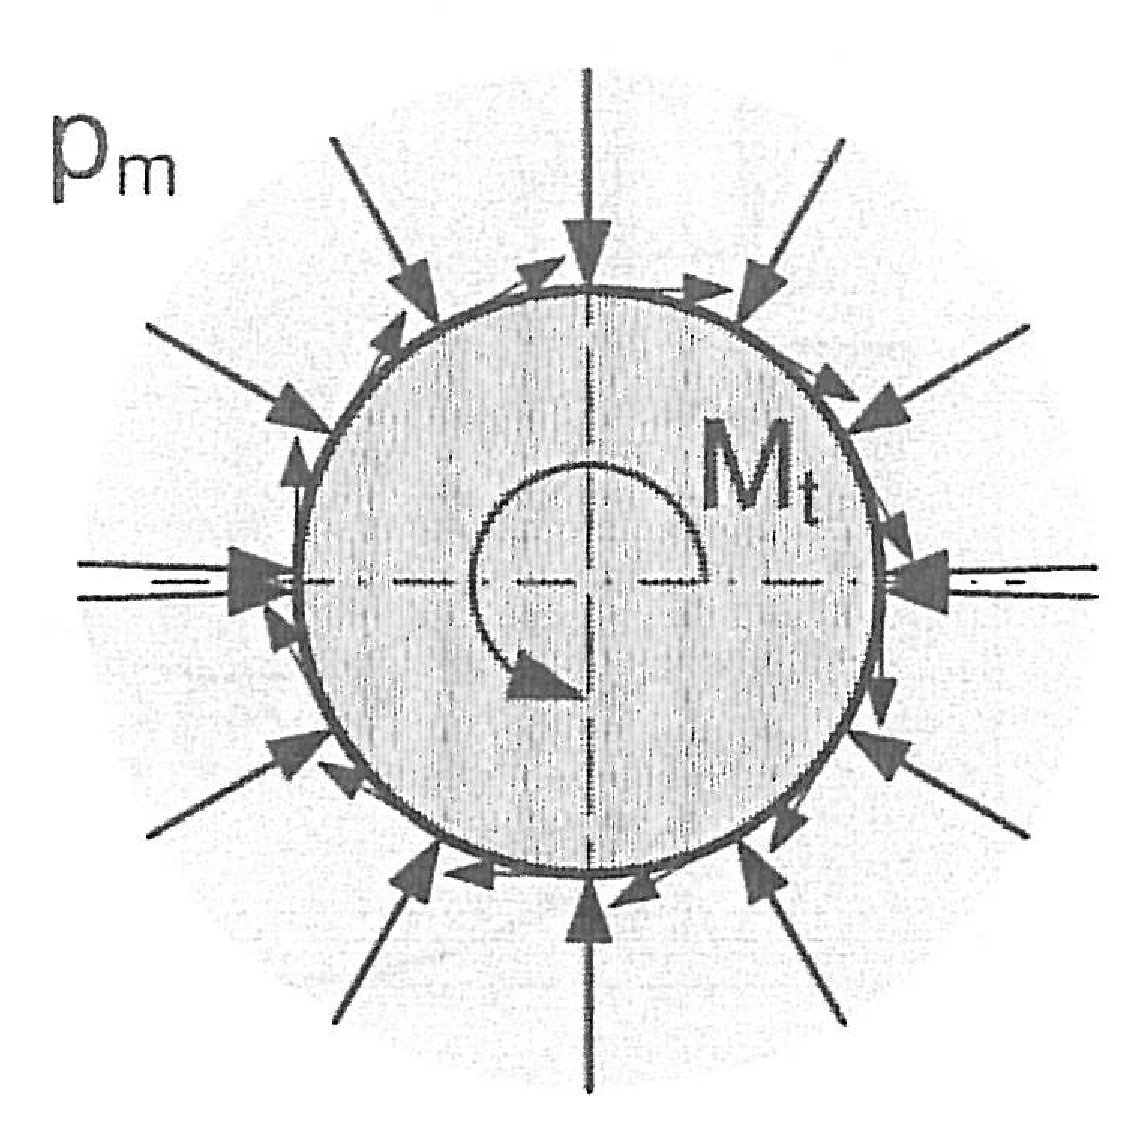
\includegraphics[width=\linewidth]{kupplungen/klemmverbindung-weich}
		\caption*{Biegeweiche Klemmverbindung}
	\end{minipage}
\end{figure}

\pagebreak
% geschlitzte Klemmverbindung
\hrule
\begin{eeqn}{geschlitzte Klemmverbindung}
	\begin{align}
		& M = 2\cdot F_\text{S} \cdot \frac{a+k}{b} \cdot \mu \cdot D_\text{F} \\
		& P = \frac{F_\text{N3}}{l\cdot D_\text{F}}
	\end{align}
	In der Verbindung treten folgende Kräfte auf:
	\begin{align}
		&F_\text{N 1,2} = S \cdot \frac{a+k}{b} \\
		&F_\text{N3} \approx 2 \cdot F_\text{N 1,2}
	\end{align}

	Für die Konstanten $a, b, k$ gelten folgende Näherungen:
	\begin{align}
		&a  \approx 0,5 \cdot D_\text{B} + 0,5 \cdot D_\text{F}+ c\\
		&c \approx 0,1 \cdot D_\text{F}\\
		&b \approx \frac{H+D_\text{F}}{4} \\
		&k \approx 0,1 \cdot D_\text{F} \qquad (k\approx 0,05 \cdot D_\text{F} \ldots  0,2 \cdot D_\text{F})
	\end{align}
\end{eeqn}

\begin{figure}[H]
	\centering
	\begin{minipage}[b]{0.48\linewidth}
		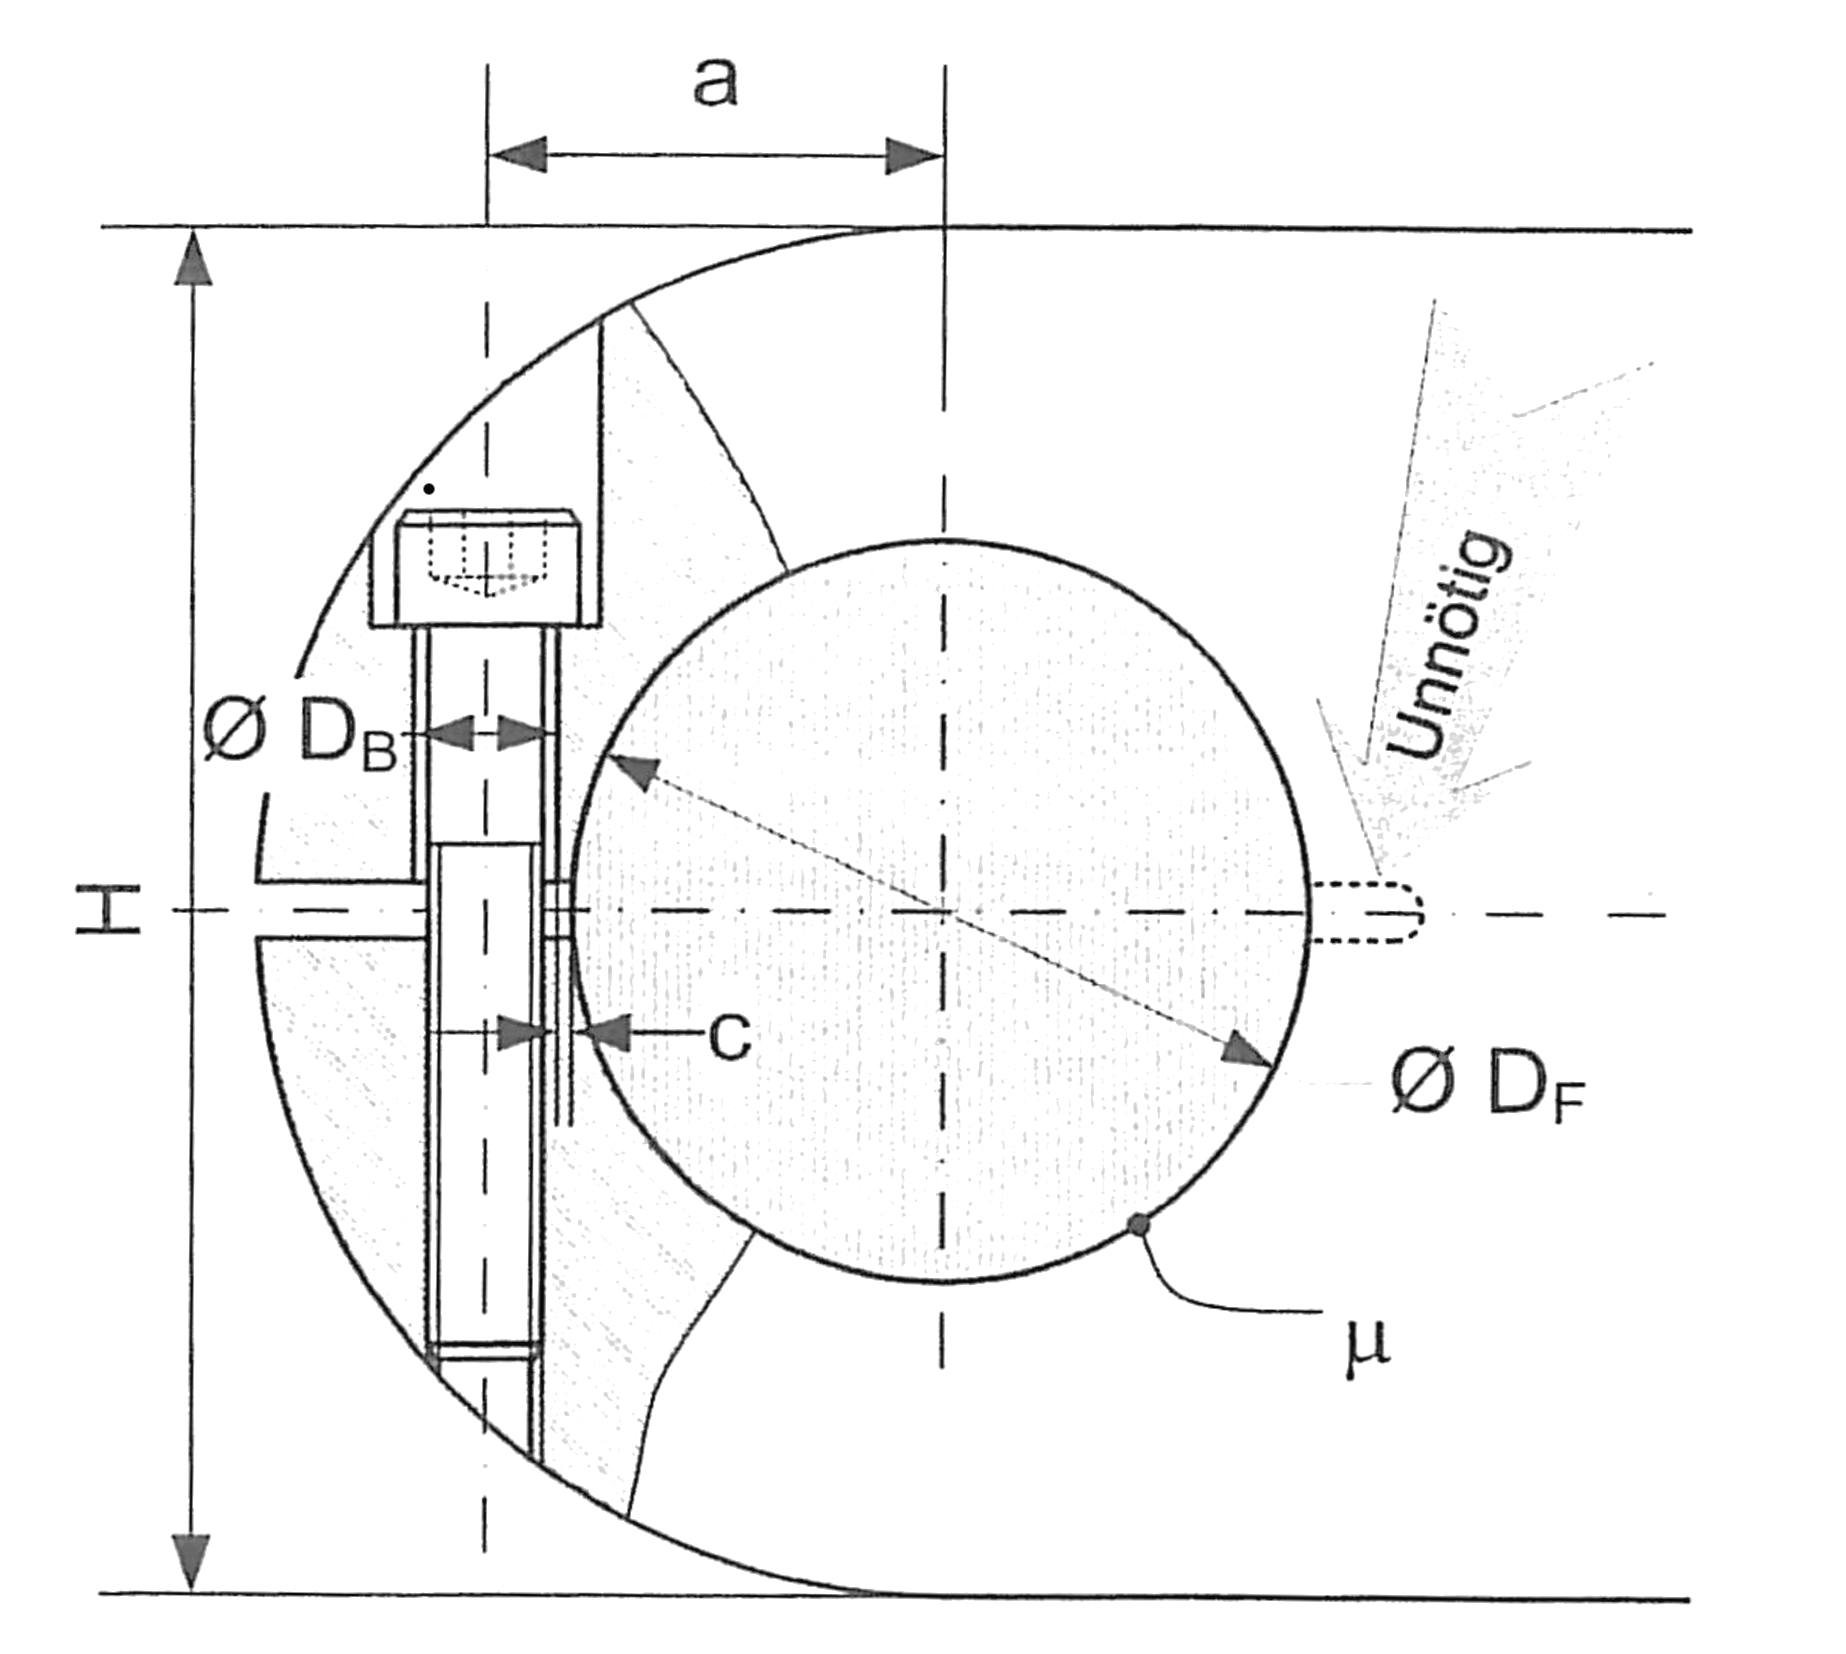
\includegraphics[width=\linewidth]{kupplungen/geschlitzte-klemmverbindung}
		\caption*{Geschlitze Klemmverbindung}
	\end{minipage}
		\begin{minipage}[b]{0.48\linewidth}
		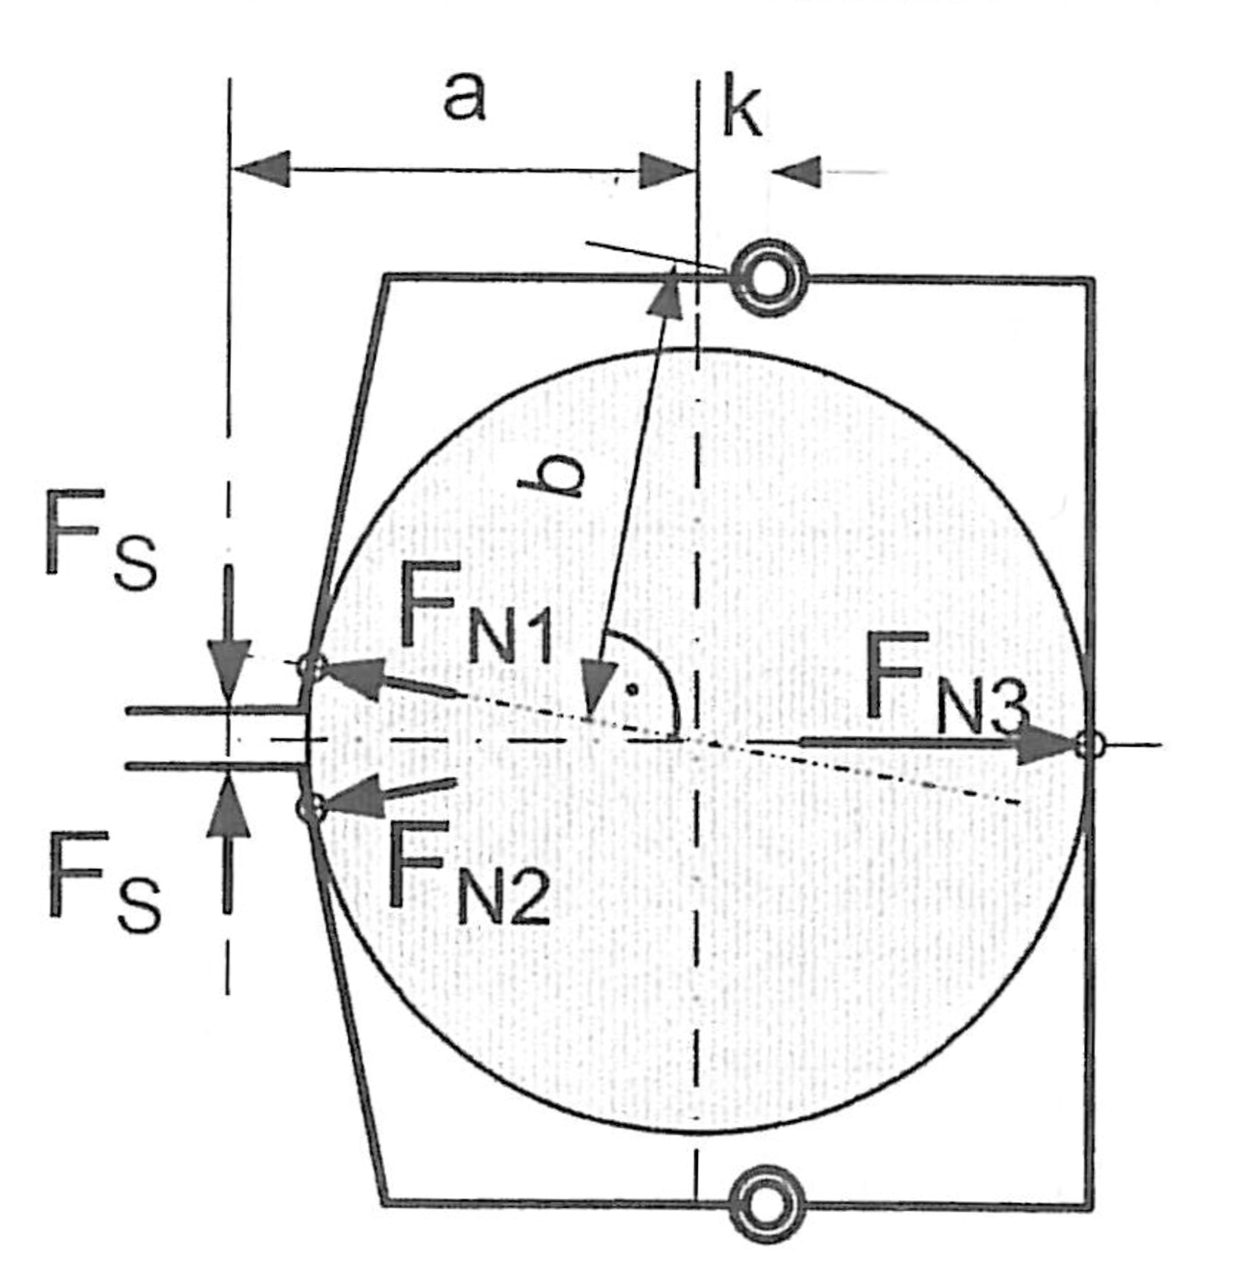
\includegraphics[width=\linewidth]{kupplungen/geschlitzte-klemmverbindung-frei}
		\caption*{Krafteinwirkung}
	\end{minipage}
\end{figure}
